% 
% Annual Cognitive Science Conference
% Sample LaTeX Paper -- Proceedings Format
% 

% Original : Ashwin Ram (ashwin@cc.gatech.edu)       04/01/1994
% Modified : Johanna Moore (jmoore@cs.pitt.edu)      03/17/1995
% Modified : David Noelle (noelle@ucsd.edu)          03/15/1996
% Modified : Pat Langley (langley@cs.stanford.edu)   01/26/1997
% Latex2e corrections by Ramin Charles Nakisa        01/28/1997 
% Modified : Tina Eliassi-Rad (eliassi@cs.wisc.edu)  01/31/1998
% Modified : Trisha Yannuzzi (trisha@ircs.upenn.edu) 12/28/1999 (in process)
% Modified : Mary Ellen Foster (M.E.Foster@ed.ac.uk) 12/11/2000
% Modified : Ken Forbus                              01/23/2004
% Modified : Eli M. Silk (esilk@pitt.edu)            05/24/2005
% Modified: Niels Taatgen (taatgen@cmu.edu) 10/24/2006

%% Change ``a4paper'' in the following line to ``letterpaper'' if you are
%% producing a letter-format document.

\documentclass[10pt,letterpaper]{article}

\usepackage{amsmath, amssymb}
\usepackage{cogsci}
\usepackage{pslatex}
\usepackage{apacite}
\usepackage{graphicx} 
\usepackage{natbib}
\usepackage{pseudocode}
\usepackage[font=small,skip=5pt]{caption}

\renewcommand{\topfraction}{0.9}	% max fraction of floats at top
\renewcommand{\bottomfraction}{0.8}	% max fraction of floats at bottom
%   Parameters for TEXT pages (not float pages):
\setcounter{topnumber}{2}
\setcounter{bottomnumber}{2}
\setcounter{totalnumber}{4}     % 2 may work better
\setcounter{dbltopnumber}{2}    % for 2-column pages
\renewcommand{\dbltopfraction}{0.9}	% fit big float above 2-col. text
\renewcommand{\textfraction}{0.07}	% allow minimal text w. figs
%   Parameters for FLOAT pages (not text pages):
\renewcommand{\floatpagefraction}{0.7}	% require fuller float pages
% N.B.: floatpagefraction MUST be less than topfraction !!
\renewcommand{\dblfloatpagefraction}{0.7}	% require fuller float pages
\setlength{\parskip}{2mm plus1mm minus0mm}
%\setlength{\textfloatsep}{\baselineskip plus 0.2\baselineskip minus 0.2\baselineskip}


\newcommand{\eg}{e.g. }
\newcommand{\ie}{i.e. }
\newcommand{\fg}{Fig.}
\newcommand{\corevectors}{core}
%\newcommand{\inverseop}[1]{\mathbf{#1}'}
\newcommand{\inverseop}[1]{\overline{\mathbf{#1}}}
\newcommand{\synset}[1]{\textbf{#1}}
\newcommand{\relation}[1]{\textbf{#1}}
\newcommand{\unbinding}{unbinding}
\newcommand{\rel}{rel}
\newcommand{\sub}{subj}
\newcommand{\obj}{obj}
\newcommand{\Sarah}{Eve}
\newcommand{\Fido}{Max}


\title{Learning Semantic Networks in Spiking Neurons}
 
%\setlength{\textfloatsep}{5pt plus 1.0pt minus 2.0pt}
\author{\large \bf Eric Crawford (e2crawfo@uwaterloo.ca)\\
  \large \bf Chris Eliasmith (celiasmith@uwaterloo.ca)\\
  Centre for Theoretical Neuroscience, University of Waterloo,
  Waterloo, ON, N2L 3G1}
\setlength{\intextsep}{1pt plus 1.0pt minus 2.0pt}
\setlength{\textfloatsep}{5pt plus 1.0pt minus 2.0pt}
%\setlength{\textfloatsep}{.1cm}
\begin{document}


%\abovedisplayskip=1pt

\maketitle

\begin{abstract}
Because it provides no straightforward characterization of stuctured knowledge, the connectionist regime generally struggles to provide a convincing account of how highly structured information can be learned and represented. A particular thorny issue with many previous attempts has been the isssue of scaling; we know humans possess massive amounts of structured knowledge (the average adult human vocabulary contains roughly 60,000 items), but no previous technique provides anywhere near the efficiency (in terms of neural resources) to store knowledge bases of that scale using a plausible number of neurons. Here, we present an approach, based on Vector Symbolic Architectures and a novel method for learning associations in spiking neurons, that does possess the necessary representational efficiency. We demonstrate its efficiency by applying it to a structure learning task, emulating children learning structure in their environment, and show via simulation that a knowledge base containing 5,000 items and relations between them can be reliably learned in biologically plausible spiking neurons. We also make a theoretical argument to the effect that our technique will indeed scale up to the full $\approx$ 60,000 items in the average adult vocabulary.

\textbf{Keywords:} 
knowledge representation; biologically plausible; scaling; neural; vector symbolic; plasticity; learning
\end{abstract}

\section{Introduction}
Learning large-scale structured representations is one of the most mysterious of human abilities. It has been a struggle to identify mechanisms by which huge knowledge bases, on the scale of a human vocabulary and larger, can be stored robustly in a neural format, a format which has been notoriously resistant to past efforts. In a previous paper, we demonstrated one approach to \textit{representing} large structured knowledge bases. Our technique was an improvement on all past efforts in this domain, in terms of both ability to scale and biological plausibility. The technique we presented there relied in large part on a large associative memory, and the efficient scaling came largely because of a technique for efficiently storing associations in a spiking neural network. However, one shortcoming of the technique was the the connection weights in the network work were computed offline using neural engineering techniques, and it was left as an open question whether such a representation could be learned in a biologically plausible way from experience. Here we directly address this issue, showing how such an associative representation can be learned in a biologically plausible manner that retains the advantageous scaling properties of the original, ``hand-coded'' approach.

The contributions of the current work are two-fold. First, we present a novel method for learning large numbers of associations efficiently in a spiking neural network. Second, we combine this method with a previous technique for encoding structured representations to create a biologically plausible method for learning large, structure-rich knowledge bases.

We begin by presenting the outline of our technique for representing structured knowledge neurally, demonstrating why an efficient associative memory is required. We then present a technique showing how such a memory can be learned in a neuron-efficient manner. We conclude by showing the results of simulations conducted using this technique, to solve a task that emulates a child learning semantic structure.

\section{Vector Encoding of Structured Knowledge}
We begin by presenting a formalism that allows the encoding of large structured knowledge bases, such as a semantic network, in a vectorial format. When combined with the Neural Engineering Framework, a principled way of representing vectors in spiking neurons, this formalism will act as a bridge between the previously disparate realms of spiking neural computation and large, structured knowledge bases.

\subsection{Holographic Reduced Representations}
Holographic Reduced Representations (HRRs) are a type of Vector Symbolic Architecture (VSA). They provide us with a means of representing structured knowledge in a vectorial format. 

To begin, we fix a dimension for our vectors. Previous investigations have shown that using 512-dimensional vectors provides sufficient representational capacity to accomodate knowledge bases containing on the order of 60,000 items,  CITATION, roughly the size of an adult human vocabulary. Then, each symbol in the vocabulary is assigned two vectors. The first vector is called an ID-vector, and acts as a unique identifier for the symbol it is assigned to. The second vector is an HRR that encodes the structured relations belonging to the symbol it is assigned to. This vector is built up in terms of ID-vectors corresponding to symbols that the current symbol is related to, using specialized operations specified by the HRR formalism.

Suppose, for example, that our vocabulary contains a symbol \textbf{dog}, and we would like the structured vector for dog to encode two facts about dogs, namely that they are members of packs, and that they are canines. Using the HRR operations of \textit{circular convolution} ($\circledast$) and \textit{vector addition} ($+$), the HRR for \textbf{dog} is given by:
\begin{align}
  \mathbf{dog} = \mathbf{isA} \circledast \mathbf{canine_{ID}} + \mathbf{partOf} \circledast \mathbf{pack_{ID}}\label{eqn:dog-sem}
\end{align}

In general, for each relation belonging to a symbol we want to represent, the HRR contains a term with the relation-type vector circularly convolved with the ID-vector for the target of the relation. All these terms are then added, allowing all this relational information to be stored in a single vector. Additionally, the dog HRR in \eqref{eqn:dog-sem} has the same dimensionsionality as each of the vectors on the right-hand side of the equation. This unique feature of HRR's has a number of desirable consequences. For instance, any brain structures we build to manipulate HRR's can expect vectors of a specific dimensionality. More importantly, this prevents the size of the vectors from undergoing a combinatorial explosion as the depth of the knowledge structure increases, permitting the representation of deeply hierarchical structures. We will now address the HRR operations in more detail to show why such a representation is useful.

What makes this useful is that \textbf{dog} preserves information about its constituents; given a query vector, we can use a third operation, \textit{deconvolution} to determine what the vector that the query vector is colvolved with in \textbf{dog}. Deconvolution amounts to performing circular convolution between the queried vector and the inverse of the query vector, denoted by an overbar. For example, if we want to extract the symbol that \textbf{dog} is related to via the \textbf{isA} relation type, we circularly convolve \textbf{dog} with $\overline{\mathbf{isA}}$:
\begin{align}
&\mathbf{dog} \circledast \overline{\mathbf{isA} }\notag\\
&=(\mathbf{isA} \circledast \mathbf{canine_{ID}} + \mathbf{partOf} \circledast \mathbf{pack_{ID}}) \circledast \overline{\mathbf{isA} }\notag\\
&=\mathbf{isA} \circledast \mathbf{canine_{ID}} \circledast \overline{\mathbf{isA} } + \mathbf{partOf} \circledast \mathbf{pack_{ID}} \circledast \overline{\mathbf{isA} }\notag\\
&\approx \mathbf{canine_{ID}} + \mathbf{partOf} \circledast \mathbf{pack_{ID}} \circledast \overline{\mathbf{isA} }\label{eqn:unbind}
\end{align}
Equation \eqref{eqn:unbind} shows that $\mathbf{dog \circledast \overline{isA}}$ is \textbf{canine} superposed with another vector which can effectively be regarded as noise. All that remains is to remove that noise, and we will discuss methods for doing so below.

\subsection{Associative Memories}
Observing equation \eqref{eqn:unbind}, we see that the result of deconvolution is not exactly what we want. It is insufficient in two ways. First, because of the other terms that are present, it is only \textit{similar to} $\mathbf{canine_{ID}}$; in other words, there is noise the must be removed. Second, $\mathbf{canine_{ID}}$ is not particularly useful on its own; it would be much more useful to have the HRR for canine, from which we could recursively extract further structural information. These problems can be solved simultaneously by an associative memory.

Associative memories typically store ordered pairs of vectors $<\xi, \eta>$. When the memory receives an input, if that input is sufficiently similar to some $\xi$, then the memory outputs the corresponding $\eta$. It is easy to see how this solves our problems if we let the $\xi$ be ID-vectors and the $\eta$ be HRR's: the associativity provides the mapping, and the fact that the input only has to be suffuciently similar to some $\xi$ solves the denoising problem. 

For example, for our miniature dog-centric vocabulary, we would store mappings between the ID-vectors for \textbf{dog}, \textbf{canine} and \textbf{pack} and their corresponding HRR-vectors. When the vector from equation \eqref{eqn:unbind} is fed into this associative memory, it will be similar to $\mathbf{canine_{ID}}$, and disimilar to $\mathbf{dog_{ID}}$ and $\mathbf{pack_{ID}}$. Consequently, the output of the associative memory will be $\mathbf{canine}$. 

Associative memories have a long history in cognitive science, with a number of cognitive architectures being completely centered around them. However, all of these have shortcomings. The remainder of this work will examine how an associative memory can be learned in spiking neurons in a biologically plausible manner, using a number of neurons that is linear in the number of stored vectors.

\section{Learning Structured Knowledge in Spiking Neurons}
We begin this section with a characterization of a framework that provides a principled approach to constructing networks of spiking neurons that represent and transform high-dimensional vectors, such as those used in the vectorial encoding of structured knowledge given in the previous section. We then show how to apply this approach to build a neural network capable of learning to associate arbitrary pairs of vectors.

\subsection{Neural Representation and Computation}
The Neural Engineering Framework (NEF) is a set of methods for building biologically
plausible models using principles for neural representation, computation and dynamics \citep{Eliasmith2003m}. 
The central idea behind the NEF is that a group of spiking neurons can represent
vectors over time, and that connections between groups of neurons can compute functions on those vectors. More precisely, a group of neurons represents any of a set of
vectors, that is, a vector space. The NEF provides a set of methods for determining
what the connections need to be to compute a given function on the vector space represented by a group of neurons.
Suppose we wish to compute the function y = f(x), where vector space x is represented in population A, and vector space y is represented in population B. To do so,
the NEF assumes that each neuron in A and B has a ``preferred direction vector.'' The
preferred direction vector is the vector (i.e. direction in the vector space) for which
that neuron will fire most strongly. Consequently, the spiking activity of every neuron in a population A can be written
\begin{align}
a_i (x) = G [\ \alpha_i e_i x\ +\ J_{bias}\ ]\label{eqn:enc}
\end{align}
where a$_i$ is the ith neuron in the population, G is the spiking neural nonlinearity, $\alpha_i$
is the gain of the neuron, e$_i$ is the preferred direction (or encoding) vector, and $J_{bias}$
is a bias current to account for background activity of the neuron. The elements in
the square brackets determine the current flowing into the cell, which then drives the
spiking of the chosen single cell model G. For computational efficiency, we employ
a leaky integrate-and-fire (LIF) model of neurons here, though the NEF can be applied for arbitrary neuron models. Equation \eqref{eqn:enc} is
referred to as an encoding equation because it describes how a vector space, in this case
x, is encoded into neural spikes. The NEF assumes a least-squares optimal linear decoding to 
reconstruct x or any nonlinear function thereof, $f(x)$. Thus, we must find the
decoders d$^f_i$ , such that
\begin{align}
E = \frac{1}{2}\int[f(x) - \sum_i a_i(x) d^f_i]^2dx\label{eqn:error}
\end{align}
is minimized. Finding the decoders in this manner then provides us with a way to
estimate any vector f(x) given the activities from the encoding equation. We can write
this as the decoding equation:
\begin{align}
\widehat{f(x)} = \sum_i a_i(x(t)) d^f_i \label{eqn:dec}
\end{align}
where N is the number of neurons in the group and $\widehat{f(x)}$ is the estimate of f(x) where x is the input driving the neurons. Recall that our purpose in defining representation of a vector space in a neural group
is to use it to compute a function between two populations. If we define the encoding
and decoding for groups A and B using equations \eqref{eqn:enc} and \eqref{eqn:dec}, we can substitute the
decoding of A into the encoding of B, thereby deriving connection weights. In addition, if the function we wish to compute is linear, we can include the relevant
linear operator in the weight equation. The weight equation for computing
any combination of linear and nonlinear functions is then:
\begin{align}
\omega_{ij} = d^f_i \alpha_j L e_j\label{eqn:weight}
\end{align}
where i indexes the neurons in group A and j indexes the neurons in B, f is any nonlinear function and L is any $D_B$ x $D_A$ linear operator, where $D_A$ and $D_B$ are the dimensionalities of the two vector spaces.

%It is worth noting that these representations and computations can be implemented to any desired precision by adding enough neurons. Specifically, the root mean-squared-error goes down as $\frac{1}{N}$ \citep{Eliasmith2003m}. One of the main concerns of this paper is to demonstrate that the operations required for representing human-scale lexical structure can be done with a reasonable number of neurons.

\subsection{Learning Associations in Spiking Neurons}
Given $N$ pairs of vectors to associate, $<\xi_k, \eta_k>$ for $k \in 1 \dots N$, the following simple algorithm implements the associative memory functionality:
 
\renewcommand{\thepseudocode}{1}

\begin{pseudocode}[ruled]{Association}{v}
  \label{alg:simple}
  sum \GETS 0\\
  \FOR k \GETS 1 \TO N\\
  \BEGIN
    scale \GETS threshold(\xi_k \cdot v) \\
    sum \GETS sum + scale * \eta_k\\
  \END\\
  \RETURN{sum}
\end{pseudocode} 

If the threshold is set correctly (which depends on the statistics of the input), \textit{scale} will be non-zero for at most one value of $k$, and the output will be either the zero vector or $\eta_k$.

%\begin{enumerate}
%\item Take the dot product of the input vector with each of the address vectors.
%\item Threshold these values (set to 0 all values below some fixed threshold).
%\item Multiply each stored vector by its corresponding thresholded value.
%\item Add all the resultant vectors together to obtain a single vector as output.
%\end{enumerate}
A network implementing a neural variant of this algorithm was employed in a previous paper, though in that paper the network's connection weights were determined offline using the NEF. In the neural version, each pair of vectors $<\xi, \eta>$ is assigned a small ($\sim$20) neural population. The encoding vectors of this population are set equal to $\xi$, and the neural tuning curves are set so that the neurons are only active if the input is sufficiently similar to $\xi$. The decoders of the population are set equal to $\eta$. The overall effect is that when a population is active, it outputs its assigned $\eta$, and the population is active if and only if the input is sufficiently similar to its assigned $\xi$. All these populations converge on a single output population, and their outputs are summed by the dendrites of that output population. In essence, each neural population computes, in parallel, one iteration of the loop in Algorithm \ref{alg:simple}.

The associative memory learned by our network employs these same principles. However, rather than computing the appropriate connection weights ahead of time, we want our network to arrive at them through training and the application of learning rules. A schematic diagram of the network is shown in \fg~\ref{fig:schematic}. We impose several assumptions on the pre-trained network. 
%First, we assume that the input population employs a relatively sparse representation; this increases the degree to which the activity of the neurons in the population is correlated with the vector that that population is representing at any given time, which, as we shall see, facilitates learning. 
First, we assume that the association population employs a sparse representation, such that only a few association neurons are active for any given input vector. Importantly, this initial sparseness is general; roughly the same number of neurons should be active for any input vector, and hence the initial network is equally well equipped to learn any set of associations. The second contraint we place on the initial network is that the connection weights between the association population and the output population are very small; the effect is that in the early stages of training, no activity in the association population is sufficient to elicit activity in the output population. We now outline methods by which the connection weights in this network of spiking neurons are modified in response to training input to produce a resource-efficient, robust associative memory.

\begin{figure}[b]
\begin{center}
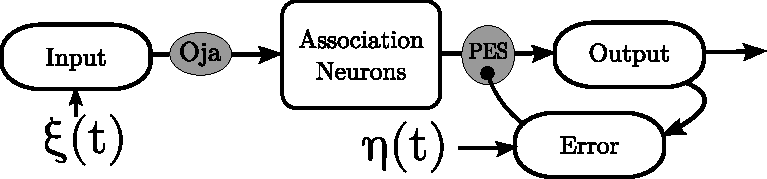
\includegraphics[width=0.5\textwidth]{../diagrams/schematic.pdf}
%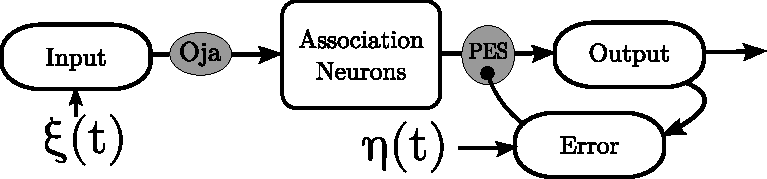
\includegraphics[width=\textwidth]{../diagrams/schematic.pdf}
\end{center}
\caption{Schematic diagram of association network. White rectangles indicate populations of spiking neurons, arrows indicate all-to-all connections between populations, and grey ellipses indicate learning rules applied to connections.}
\label{fig:schematic}
\end{figure}
\subsubsection{Training}
During training, the network has two inputs: $\xi$, the address vector, and $\eta$, the vector to be associated with $\xi$. We present each pair that we want our network to store for one second of simulation time, and allow the network to adjust its connection weights.

\subsubsection{Sparse Representation}
The initially sparse representation in the association layer ensures that only a few association neurons are active for any vector presented during training. These active neurons can be thought of as the neurons assigned to that pairing. With the above algorithm in mind, the goal, then, is to set the encoders of this population equal to $\xi$, and set the decoders of this population equal to $\eta$, using biologically plausible learning rules. 

\subsubsection{Oja's Rule: Increasing Selectivity}
The first step is to make the active association neurons more selective for the current $\xi$. This may seem redundant, as the sparse representation ensures that the neurons are already fairly selective for the current input vector. However, those active neurons will also respond to other vectors that we might try to store in our memory, which could cause multiple association populations to become active when the memory is used. Our goal here is to ensure that these neurons are active only for input vectors that have a high-degree of similarity to the current training vector. Once training is complete, we want it to be the case that this population is active if and only if the input is a noisy version of the vector the population is assigned to, and thus will have no effect on the output if that is not the case.

To achieve this increase in selectivity, we use a normalized hebbian learning rule known as Oja's Rule. The ``normalized'' feature of the rule ensures that the connection weights do not grow arbitrarily, which is a major shortcoming of hebbian learning in its simplest form. The weight-update equation employed by Oja's rule is:
\begin{align}
  \Delta w_{ij} = \alpha (x_i y_j - \frac{y_j^2 w_{ij}}{\beta})
\end{align}
where $x_i$ is the activity of the $i$th neuron in the input population, $y_j$ is the activity of the $j$th association neuron, $\alpha$ is a constant corresponding to the learning rate, and $\beta$ is a constant that is asymptotically proportional to $\sum_i w_{ij}^2$, the sum of squares for each row of the weight matrix. Because the neurons are spiking, the activities $x_i$ and $y_j$ are low-pass filtered versions of spike trains. Fig. \ref{fig:oja} shows an example of what can be achieved by Oja's rule. The effect is to increase connection weights between neurons on the input population that are currently active, and active association neurons. During presentation of a noisy version of that same vector, many of the same input neurons will be active, which should be sufficient to activate the association neurons.

\begin{figure}[ht]
\begin{center}
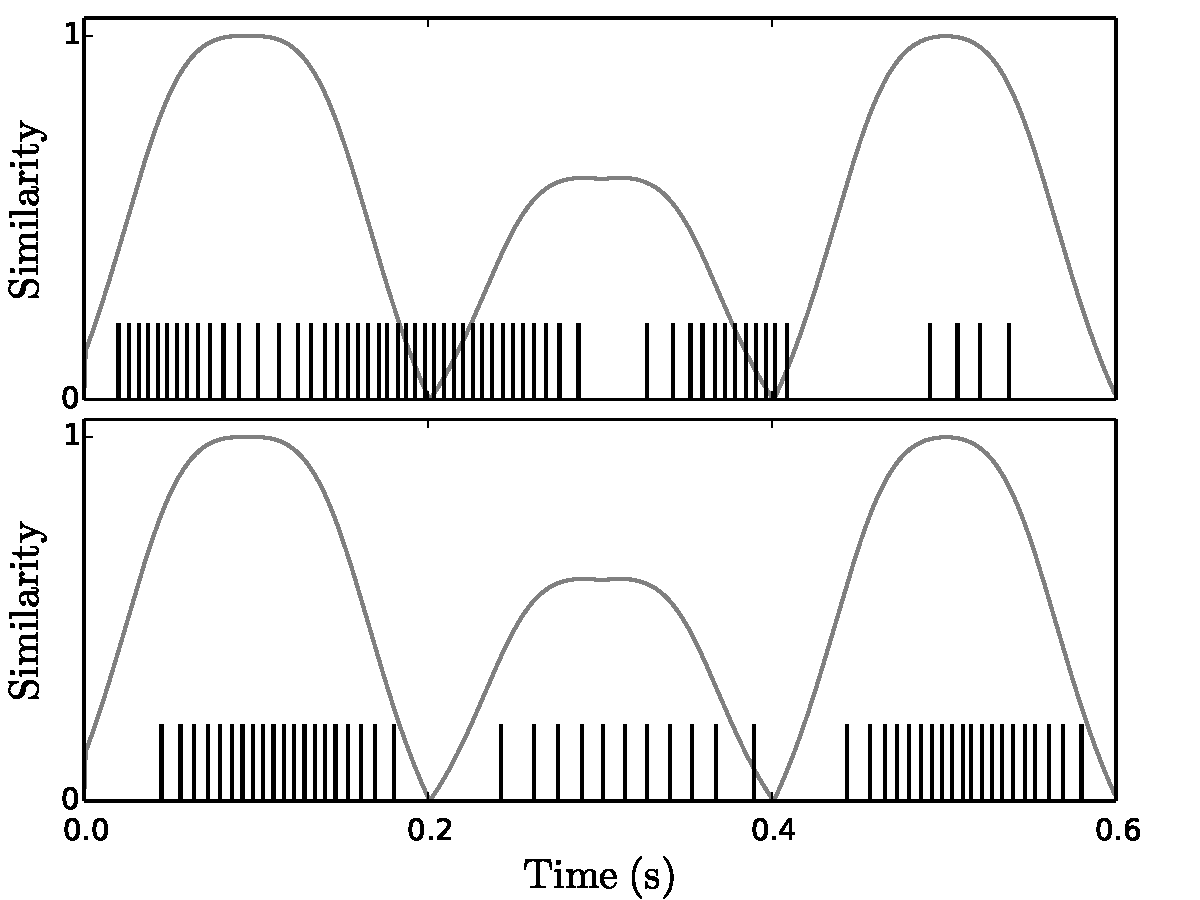
\includegraphics[width=0.5\textwidth]{../plots/oja_plot_D_64.pdf}
\end{center}
\caption{Oja's rule changes neural selectivity. A population of neurons capable of representing a 64 dimensional vectors is connected to a single association neuron. Training phase: connection weights between population and association neuron changed according to Oja's rule while population represents a training vector. Gray line shows similarity of input to the training vector during a test phase, spike raster is the response of the association neuron. (Top) Before training. (Bottom) After training. The assocation neuron has become selective for the training vector.}
\label{fig:oja}
\end{figure}

\subsubsection{Prescribed Error Sensitivity: Storing Vectors in Connection Weights}
Increasing selectivity of active neurons gets us part of the way. What we require from here is a way of setting the decoders of the active neurons to $\eta$. For this we use a supervised learning rule known as Prescribed Error Sensitivity (PES). CITATION macneil and eliasmith. 
\begin{align}
\Delta \omega_{ij} = \kappa \alpha_j \mathbf{e_j} \cdot \mathbf{E}a_i
\end{align}
where $\kappa$ is a scalar learning rate, $E$ is a vector giving the error that we want to minimize, and $a_i$ is the vector of activities of the association neurons. $E$ is the supervision signal, and represents the difference between the vector that the output population is currently representing, and the vector it ``should'' be representing, in this case $\eta$ of the current training pair. The rule essentially works to minimize $E$ by changing the connection weights between of the active neuron in the association population and neurons in the output population. This rule has been used to learn connection weight matrices that compute complicated non-linear functions; in particular, it has successfully used to learn the circular convolution operation required for manipulating HRRs. Here we are learning what amounts to constant function (during the presentation of a single pair), which is well within the capabilities of the rule.

\section{Simulations}
To test the efficacy of our network, we apply it to the task of learning structured knowledge bases, represented as randomly-generated directed graphs with small-world, scale-free structure, as there is evidence that semantic networks in general have these properties \citep{Tenenbaum2005}. If the nodes are taken to correspond to semantic elements, and the edges to correspond to relations between those elements, then the network can be interpreted as learning semantic structure, superficially similar to a child learning the structure of his environment.

We begin each trial by creating a scale-free directed graph with a certain number of nodes, and use the HRR formalism to create a vector encoding of the graph, assigning each node an ID-vector and an HRR storing its relations. We present each ID-vector/HRR pairing to the network for 1 second of simulation time, allowing the network to change its connection weights. Keeping the analogy of a child learning the stucture of their environment, we can think of this as the child having used context and the many other faculties at their disposal to determine the relations of some term to terms that it already knows, this is the creation of the structured HRR vectors. In presenting the pair to our network, the child's brain is attempting to store this structure it hsa learned in long-term memory.

To assess the learned network, we perform two sets of tests. In the first, we randomly pick and edge from the graph that the network is supposed to have learned, and test whether it has encoded it. This amounts to taking the HRR vector for the node at the tail of the edge, deconvolving it offline with the appropriate edge vector, and feeding the result into the learned network. If the network has learned the edge correctly, then it should output the HRR vector for the node at the head of the edge. The fact that the deconvolution is done offline, and not in neurons, is not an issue, as it has been shown elsewhere that spiking networks performing these operations can indeed be learned. The second test assesses whether the network has encoded the graph with sufficient fidelity such that it can be used to decode entire paths through the graph. For this, we randomly choose a directed path through the graph of length 3. We begin by performing the same operation as in the previous test on the first node in the path. In this case, however, rather than stopping there, we take the vector output by the graph, normalize it, and recursively perform the same operations on it, until the network should have arrived at the last node in the path. We take the vector output by the network at this point and compare it to the HRR vector for the last node in the path. 

%The memory works best if eta is assumed to be random, or to have undergone pattern separation to some extent.  nu is assumed to store structural relations. 
%It is worth taking a moment to consider where such a structured representation might come from in a child. There is considerable evidence that children are able to use myriad environmental and social cues, combined with strategies that are likely hard-coded in through evolution, to determine the referents of words. They may even use this structure as its built to determine context for learning new concepts. We assume that such faculties have been employed to create the vector nu storing the relational information. The primary role of our network, then, is to \textbf{store} these relations. 

\begin{figure*}[ht]
\begin{center}
\includegraphics[width=\textwidth]{../plots/example_plot_D_32_N_5.pdf}
\end{center}
\caption{An example simulation. The network learns to associate 5 pairs of 64-dimensional vectors. Before 5 seconds is the training period, after 5 seconds is the testing period. The test vectors are noisy versions of the training vectors. Notice that roughly the same set of neurons is active during the testing as during training. There are extra neurons active during training, but generally those neurons have not be ``assigned'' to any other vector pair, and hence their decoders are set to 0 and have essentialy no effect on the output. Neurons that have been assigned to other vectors are generally less active due to the increased selectivity caused by Oja's rule.}
\label{fig:example}
\end{figure*}

\section{Discussion}

\subsection{Scaling}
The primary advantage of our method for encoding structured knowledge is its ability to scale up. Consequently, for the current work to count as an improvement, the scaling properties should be retained. However, the significant additional computation introduced by the learning rules currently prevents us from running simulations where the network learns to encode a semantic network on the scale of a human vocabulary. Instead, we demonstrate that our approach at least works on more modestly sized semantic networks, and present a theoretical argument suggesting that the number of neurons required will always been linear in the number of vectors we store. 

\subsection{Future Work}
The current study leaves a number of questions unanswered. Future work will investigate whether the learned memory can be mapped to brain structures. Moreover, work will be done to investigate the time course on which presentations to the network should occur, to adhere to data about the manner and rate in which children learn such relations. It would be interesting to see whether different time courses have consequences for what is ultimately learned by the memory. For instance, there is reason to expect such a memory to be able to account for interference effects; if a new item is learned while a similar item is still being recorded, it is a plausible hypothesis that, through Oja's rule, the new item will ``steal'' neurons from the incomplete item, rendering the incomplete item difficult or even impossible to access. This has been observed empirically CITATION. Further simulations will be required to investigate these intriguing questions.

Provides certain self-correcting mechanism.
Moreover.. if you learn one relation at some early point, but then never see that relation again, but do see many other relations, the old one could be cancelled out, which could ultimately be a good thing.. the original one could be cancelled out over time.

One shortcoming of our method is that there is a limit to the number of relations that can be stored in any given vector. This is a consequence of the fact the HRR's compress many vectors of a given dimension into a single vector of the same dimension; obviously if we try to stuff too many vectors into a single HRR, much of the information will be lost. This seems like an important shortcoming, since clearly it is possible to know quite a lot about a given subject; experts abound. Our answer to this challenge is that since our method is so efficient, it is possible to have many of these memories in the brain. Thus as one becomes an expert in a subject, their representations of items will become more fine-grained, all these subtle distinctions being offloaded to another memory in a separate part of the brain. This may explain the commonly observed phenomena that experts have larger brains and more neurons in brain areas that are known to be relevant to their area of expertise CITATION.

%Pattern separation and the identity vectors.
Further explication the form of semantic representations in the brain.. i.e. emprically determing WHAT gets stored. i.e., what exactly are the identity vectors? seems like an important question.

%Role of neurogenesis, so we don't need a predetermined size of the cleanup pool. 
%Our network can potentially also be seen as playing a role in determining what actually gets learned as well. 
%Further, our network permits single relations to be learned at a time, while still permitting the entire structure to be accessed later on. This seems more plausible, as it is obviously not the case that children learn all properties relations of a word in a single blush.

%Network basically requires that when adding relations, has to be relations to something we already know about, or is already in our memory. This is in accordance with how things are done in wordnet.. its likely that general categories are learned before specific (i.e. entity before dog before wolfhound), and since the predominant relation is isA, wolfhound has to be added after dog anyway.



\section{Conclusion}
Novel combination of synaptic plasticity and distributed vector representations. 

\section{Acknowledgments}
Funding for this work was provided by the National Science and Engineering Research Council of Canada, Canada Research Chairs, the Canadian Foundation for Innovation and the Ontario Innovation Trust.		
\bibliographystyle{apacite}

\setlength{\bibleftmargin}{.125in}
\setlength{\bibindent}{-\bibleftmargin}

\bibliography{library}

\end{document}
